\chapter{Datasets} \label{sec:ch_data}

\graphicspath{{../img/ch40/}}



In this chapter several datasets will be described. The datasets can be divided into several groups according to several criterions: 
\begin{itemize}
	\item structure and purpose of a particular dataset (textual for IE tasks, relational for classification ML tasks and RDF datasets for Semantic Web reasoning tasks), 
	\item presence of manual annotations,
	\item language in case of textual data (English and Czech), 
	\item the origin of the dataset (third party datasets and datasets created as a part of the presented work).
\end{itemize}
The description of individual datasets will be presented at the very end of the chapter, before that, relevant common aspects of the datasets will be discussed.


\section{Purpose and Structure}
In this section a distinction of datasets according their purpose and structure will be presented. Three types of datasets will be discussed: Information Extraction Datasets, Classification Datasets and Reasoning Datasets.

\subsection{Information Extraction Datasets}
An IE dataset is made up of a set of text documents. The texts are usually manually annotated (with one exception see Section~\ref{sec:ch40_fireman_without}). The manual annotations are of the form of labels on shorter segments of the text (the length of a segment ranges between one to approximately three tokens). 

An IE engine can use such dataset for training and evaluation. During evaluation, the dataset is split into two parts -- training set and testing set. An IE engine is trained on the training set and success is measured on testing set by comparing the annotations returned by the IE engine and the actual annotations present in the dataset.
Performance measures of precision and recall are mostly used for evaluation. 

Following datasets can be regarded as IE datasets:

\begin{itemize}
	\item \sectiondoubleref{sec:ch40_fireman_without}
	\item \sectiondoubleref{sec:ch40_fireman_annotated}
	\item \sectiondoubleref{sec:ch40_corporate_acquisitions}
\end{itemize}




\subsection{Reasoning Datasets}

%Guo, Yuanbo, Heflin, Jeff and Pan, Zhengxiang . Benchmarking DAML+OIL Repositories. Second International Semantic Web Conference, ISWC 2003, LNCS 2870. Springer. 2003. pp.613-627.

The term ``Reasoning Datasets’’ is used here for the type of datasets which are used in Ontology Benchmarks. Ontology benchmarking is a scientific topic that is almost as old as ontologies and Semantic Web itself \citep{DBLP:conf/semweb/GuoHP03}. Ontology Benchmarks serve for evaluation of ontology systems and their capabilities. There are two obvious objectives of ontology benchmarking. The first one is to verify capabilities of a tested system -- weather the system is able to perform all actions prescribed by the particular benchmark. The second objective is to measure the time performance of the system. Unlike the previous two dataset types in the case of ontology benchmarking and reasoning datasets it does not make any sense to measure success of a system because there is no uncertainty in reasoning tasks. A system is either able to perform a particular action or not; it is unnecessary to measure that. 

Reasoning datasets used in the present work:
\begin{itemize}
	\item \sectiondoubleref{sec:ch40_rdf_fireman}
	\item \sectiondoubleref{sec:ch40_rdf_acquisitions}
\end{itemize}

These datasets were used for evaluation of the idea of shareable extraction ontologies, see Section~\ref{sec:ch70_experiment}. 


\subsection{Classification Datasets}
Classification datasets are very familiar in the community of machine learning. They are used for evaluation of propositional ML engines (like Decision Trees, Naive Bayes, Multilayer Perceptron, Support Vector Machines, etc.) on the classification task. The classification task (or problem) can be simplified way described as follows: 

Given a set of objects (e.g. accidents); each object is described using a fixed set of attributes (e.g. number of fatalities, number of injuries, number of intervening units; etc.) and each object is classified into one of a fixed set of classes (not serious accident, middle serious accident, very serious accident). Based on the known classification of the objects (training set), predict the classification for new objects that have been not classified yet (testing set). 

A classification dataset is made up of a relational table. Each row of the table represents a single object; each column of the table represents a single attribute. One attribute (column) is marked as a class attribute and the values of this attribute determine the target classification. 

Similarly to the previous section, the dataset is split into two parts during the evaluation. A ML engine is trained on the training set and success is measured on testing set by comparing the predicted classification of the ML engine and the actual classification present in the dataset.

Classification datasets used in the present work:
\begin{itemize}
	\item \sectiondoubleref{sec:ch40_classify_fireman}
	\item \sectiondoubleref{sec:ch40_uci_datasets}
\end{itemize}

These datasets were used for evaluation of the Fuzzy ILP classification method in Section~\ref{sec:ch80_eval}. 




\section{Origin of the Datasets}
The datasets can be simply divided into third party and contributed. 

\subsection{Contributed Datasets}
Datasets that were partly or mostly prepared as a part the present work are:


\begin{itemize}
	\item \sectiondoubleref{sec:ch40_fireman_without}
	\item \sectiondoubleref{sec:ch40_fireman_annotated}
	\item \sectiondoubleref{sec:ch40_rdf_fireman}
	\item \sectiondoubleref{sec:ch40_rdf_acquisitions}
	\item \sectiondoubleref{sec:ch40_classify_fireman}
\end{itemize}

All the contributed datasets can be downloaded from the web site of the project. 
\subsection{Third Party Datasets}

Datasets that were used without any additional contributions are:

\begin{itemize}
	\item \sectiondoubleref{sec:ch40_corporate_acquisitions}
	\item \sectiondoubleref{sec:ch40_uci_datasets}
\end{itemize}


\section{Individual Datasets}
In this section individual datasets used in this thesis will be presented. The order of dataset presentations is the same as the order in which they were used in our work.

\subsection{Czech Fireman Reports without Annotations} \label{sec:ch40_fireman_without}
In the early beginning of our work, first IE experiments were done with textual reports from fire departments of several regions of the Czech Republic. These departments are responsible for rescue and recovery after fire, traffic and other accidents. Likewise the reports do not deal only with fire and traffic accidents but also chemical interventions, fire-fighting contests, fire drills and similar events can be found. The reports are rich in information, e.g. where and when an accident occurred, which units helped, how much time it took them to show up on the place of accident, how many people were injured, killed etc. An example of such report can be seen in the Figure~\ref{fig:ch50_article}.

The dataset is made up by 814 texts of the reports collected in the time period from February to September 2007 using a RSS feed. All the reports are still available on the web site of the Ministry of Interior of the Czech Republic\footnote{\url{http://www.hzscr.cz/hasicien/}}. 

Following URL pattern can be used to obtain a particular report:


\begin{center}
\verb+http://aplikace.mvcr.cz/archiv2008/rs_atlantic/hasici/REGION/ID.html+
\end{center}

For example report 47443 (ID) from Jihomoravský region has following URL:

\begin{center}
\verb+http://aplikace.mvcr.cz/archiv2008/rs_atlantic/hasici/jihomoravsky/47443.html+
\end{center}


The dataset contains reports from eight Czech regions: Jihomoravský (127 reports), Královéhradecký (109 reports), Moravskoslezský (138), Olomoucký (77), Pardubický (95), Plzeňský (97), Ústecký (108) and Vysočina (63). All the reports are written in Czech language. 

The dataset does not contain any manual annotations; only linguistic annotations produced by PDT tools are included in the dataset (FS format for Netgraph processing and PML format for Btred processing, see Section~\ref{sec:ch30_pdt_tools_and_resources} for details about these tools). Table~\ref{tab:ch40_fire_without} summarizes some properties of the dataset’s reports described bellow.  Total sum, average value, standard deviation, minimum, maximum and median of the values can be found in the table.


Text size is the length of the text of a particular report in characters. More precisely it is the size of the corresponding ``.txt'' file. ISO-8859-2 (Latin-2) character encoding is used in these files so the number of characters is the same as the file size in bytes. 

Number of words in a particular report is counted using UNIX command ``wc -w''.

Annotations size expresses the number of bytes used by the corresponding linguistic annotations of a particular report. Only annotations in FS format are counted (PML files are not included in these numbers).

Number of trees is the number of tectogrammatical trees in a particular report. The number also corresponds with the number of sentences in the report.


The dataset was used for a quantitative evaluation experiment described in Section~\ref{sec:ch50_quant_experiment}. 


\begin{table}
\centering
\begin{tabular}{|l|r|r|r|r|r|r|}
\hline
 & sum & avg & st. dev. & min & max & median\\
\hline
text size    &  1 298 112 &  1 594.7 &  1 142.34 &    57 &  11 438 &  1 290.5\\
num. words   &    195 168 &    239.8 &    172.02 &     9 &   1 750 &    193.0\\
annot. size  & 51 464 581 & 63 224.3 & 43 557.61 & 4 648 & 451 953 & 52 033.5\\
num. t-trees &     15 208 &     18.7 &     15.02 &     1 &     143 &     14.0\\
\hline
\end{tabular}
\caption{Dataset \ref{sec:ch40_fireman_without} -- \nameref{sec:ch40_fireman_without} -- statistics} \label{tab:ch40_fire_without}
\end{table}


\subsection{Czech Fireman Reports Manually Annotated} \label{sec:ch40_fireman_annotated}

We have created a manually annotated version of the previous dataset. 
This dataset was created by ourselves during the development of our IE  engine based on machine learning (Section~\ref{sec:methods_learning}). 50 reports from the previous dataset were selected and manually annotated. 
 Several annotation types were used; numbers of annotations per each annotation type are summarized in Table~\ref{tab:ch40_fire_with} along with the information whether the particular annotation type was used in the evaluation. See details abut the evaluation results in Section~\ref{sec:eval_learning}. 



>>>Event extraction?

>>>>>>>>>Vlozip popis jednotlivych typu informace<<<<<<

\begin{table}
\centering
\begin{tabular}{|r||c|c|}
\hline
\textbf{annotation type} & \textbf{number of annotations} & \textbf{used in evaluation}\\
\hline
\hline
profesional\_unit & 78 & yes\\
\hline
cars & 45 & no\\
\hline
end & 42 & no, end\_subtree only\\
\hline
end\_subtree & 42 & yes\\
\hline
start & 42 & yes\\
\hline
injuries & 33 & yes\\
\hline
amateur\_unit & 31 & yes\\
\hline
damage & 20 & yes\\
%\hline
%damageNumber & 20 & yes\\
\hline
pipes & 16 & no\\
\hline
profesional\_units & 14 & yes\\
\hline
fatalities & 11 & yes\\
\hline
units & 10 & no\\
\hline
aqualung & 8 & no\\
\hline
duration & 3 & no\\
\hline
fan & 3 & no\\
\hline
amateur\_units & 1 & no\\
\hline
lather & 1 & no\\
\hline
\end{tabular}
\caption{Dataset \ref{sec:ch40_fireman_annotated} -- \nameref{sec:ch40_fireman_annotated} -- manual annotations} \label{tab:ch40_fire_with}
\end{table}








\subsection{Corporate Acquisition Events} \label{sec:ch40_corporate_acquisitions}

\begin{table}
\centering
\begin{tabular}{|r||c|c|}
\hline
\textbf{annotation type} & \textbf{number of annotations} & \textbf{used in evaluation}\\
\hline
\hline
acqabr & 1450 & maybe\\
\hline
acqbus & 264 & no\\
\hline
acqcode & 214 & no\\
\hline
acqloc & 213 & no\\
\hline
acquired & 683 & yes\\
\hline
dlramt & 283 & yes\\
\hline
purchabr & 1263 & maybe\\
\hline
purchaser & 624 & yes\\
\hline
purchcode & 279 & no\\
\hline
seller & 267 & yes\\
\hline
sellerabr & 431 & maybe\\
\hline
sellercode & 136 & no\\
\hline
status & 461 & no\\
\hline
\end{tabular}
\caption{Dataset \ref{sec:ch40_corporate_acquisitions} -- \nameref{sec:ch40_corporate_acquisitions} -- manual annotations} \label{tab:ch40_acquisitions}
\end{table}


The second manually annotated information extraction dataset used in this thesis is called ``Corporate Acquisition Events''. It was originally described by \cite{lewis1992representation}, but, more precisely, we use the \emph{Acquisitions v1.1} version\footnote{This version of the corpus comes from the Dot.kom (Designing infOrmation extracTion for KnOwledge Management) project's resources: \url{http://nlp.shef.ac.uk/dot.kom/resources.html}} of the corpus.
It is a collection of 600 news articles describing acquisition
events taken from the Reuters dataset. News articles are tagged to identify fields
related to acquisition events. These fields include `purchaser' , `acquired', and
`seller' companies along with their abbreviated names (`purchabr', `acqabr' and
`sellerabr'). Some news articles also mention the field `deal amount'. 
Table~\ref{tab:ch40_acquisitions} provides numbers of annotations per annotation type for the whole dataset along with the information whether the particular annotation type was used in the evaluation. See details abut the evaluation results in Section~\ref{sec:eval_learning}. 



\subsection{RDF Dataset Based on Czech Fireman Reports} \label{sec:ch40_rdf_fireman}

Both reasoning datasets presented in this work are based on information extraction tasks. The datasets were created for evaluation of the idea of shareable extraction ontologies (see Section~\ref{sec:methods_Shareable_Extraction_Ontologies}). The datasets consists of so called document ontologies -- RDF representation of source documents (see Section~\ref{sec:ch70_doc_ont}) and extraction ontologies -- RDF representation of extraction rules (see Section~\ref{sec:ch70_extraction_ontologies}). Besides that there are also small mapping ontologies that solve small differences of the schemas used in document and extraction ontologies.

The reasoning task is to combine the three kinds of ontologies and infer all instances that should be found by the extraction rules saved in the particular extraction ontology, for details see the Section~\ref{sec:ch70_experiment}.

This dataset is based on the IE dataset \sectiondoubleref{sec:ch40_fireman_annotated}; it consists of 50 document ontologies, one mapping ontology and currently one extraction ontology, which contains extraction rules for the `damage' task -- to find an amount (in CZK - Czech Crowns) of summarized damage arisen during a reported accident.

Section~\ref{sec:ch70_datasets} provides also some additional information (basic statistics) about the dataset.


\subsection{RDF Dataset Based on Corporate Acquisition Events} \label{sec:ch40_rdf_acquisitions}

This is the second reasoning dataset presented in this work. The dataset is very similar to the previous one (see details in the previous section). It is based on the information extraction dataset \sectiondoubleref{sec:ch40_corporate_acquisitions}. It consists of 600 document ontologies, one mapping ontology and currently one extraction ontology, which contains extraction rules for the `acquired' task.

Section~\ref{sec:ch70_datasets} provides also some additional information (basic statistics) about the dataset.



\subsection{Classification Dataset Based on Czech Fireman Reports} \label{sec:ch40_classify_fireman}

The development of the Fuzzy ILP Classifier was partly motivated by the possibility of doing seriousness classification of accidents presented in the reports described in previous sections. We selected the same collection of 50 web reports as in the previous section and we manually extracted values of the most interesting features (These features will be described in Section \ref{sec:ch40_features}.) We also assigned a value of overall ranking of seriousness of the presented accident to each report.  The value of seriousness ranking is the target attribute of the classification task. 

%The main experiment presented in this chapter leads to the . %Our long term goal is extraction of semantic information from web reports. 
%which is one of possible utilizations of the extracted information. 
%We use online fire department reports from several regions of the Czech Republic. These reports are written in Czech and can be accessed through the web of the General Directorate of the Fire and Rescue Service of the Czech Republic\footnote{\url{http://www.hzscr.cz}}. 
%These reports are rich in information, e.g. where and when an traffic accident occurred, which units helped, how much time it took them to show up on the place of accident, how many people were injured, killed etc.

%For our experiment  We have identified several  and .  

%In this experiment we have not used any information extracted by our automated information extraction tools. Instead, we concentrate on~the classification; the actual source of the information is not so important. The integration step still lies ahead.

%There are two objectives to do. Fist is the web information extraction, a long path starting with web crawling and resulting with the extracted structured information. Second is the seriousness classification, which utilizes the extracted information. We have made much work on the first (see e.g. %\citep{biblio:DeVoLinguisticextraction2008,biblio:DeVoComputingaggregations2008, biblio:DeEcExperimentswith2008}), in this paper we will concentrate on the second.
%\citep{biblio:DeEcExperimentswith2008}), in this paper we will concentrate on the second.




\begin{table}
\centering
\begin{tabular}{|r||c|c|c|}
\hline
attribute name & distinct values & missing values & monotonic\\
\hline
\hline
size (of file) & 49 & 0 & yes\\
\hline
type (of accident) & 3 & 0 & no\\
\hline
damage & 18 & 30 & yes\\
\hline
dur\_minutes & 30 & 17 & yes\\
\hline
fatalities & 4 & 0 & yes\\
\hline
injuries & 5 & 0 & yes\\
\hline
cars & 5 & 0 & yes\\
\hline
amateur\_units & 7 & 1 & yes\\
\hline
profesional\_units & 6 & 1 & yes\\
\hline
pipes & 7 & 8 & yes\\
\hline
lather & 3 & 2 & yes\\
\hline
aqualung & 3 & 3 & yes\\
\hline
fan & 3 & 2 & yes\\
\hline
ranking & 14 & 0 & yes\\
\hline
\end{tabular}

\caption{Accident attributes.}
\label{img:ch40_attributes_description}
\end{table}


%%%%%%%%%%%%%%%%%%%%%%%%%%%%%%%%%%%%%%%%%%%%%%%%%%%%%%%%%%%%%%%%%%%%%%%%%%%%%%%%%%%%%%%%%%%%%%%%%
\subsubsection{Features of accidents} \label{sec:ch40_features}
%%%%%%%%%%%%%%%%%%%%%%%%%%%%%%%%%%%%%%%%%%%%%%%%%%%%%%%%%%%%%%%%%%%%%%%%%%%%%%%%%%%%%%%%%%%%%%%%%


Table~\ref{img:ch40_attributes_description} summarizes all features (or attributes) that were obtained from accident reports. Except for the attribute \verb+type+ (type of an accident -- \verb+fire+, \verb+car_accident+ and \verb+other+), all the attributes are numeric and therefore \emph{monotonizable} (This is important, because only monotonizable attributes can be translated to fuzzy degrees.) There are cases in which the value of an attribute is unknown. We decided to make evidence of this and keep the values \verb+unknown+ in the knowledge base. A brief explanation of each attribute follows.
\begin{itemize}
	\item \verb+size+ is length of text of a particular report.
	\item \verb+damage+ is an amount (in CZK -- Czech Crowns) of summarized damage arisen during a reported accident.
	\item \verb+dur_minutes+ is time taken to handle an accident.
	\item \verb+fatalities+ and \verb+injuries+ are numbers of deaths and wound people sustained in an accident.
	\item \verb+cars+ is the number of vehicles damaged during an accident (mostly during car accidents).
	\item \verb+professional_units+ and \verb+amateur_units+ are numbers of fireman and volunteer units sent for a particular accident.
	\item \verb+pipes+ is a number of used fire hoses.
	\item \verb+lather+, \verb+aqualung+ and \verb+fan+ (ventilator) indicates whether these devices were used.
\end{itemize}

A majority of accidents are of the type \verb+fire+ (52\%)
and \verb+car_accident+ (30\%),
the rest (type \verb+other+, 18\%)
deals with ecological disasters, chemical accidents, etc.

%%%%%%%%%%%%%%%%%%%%%%%%%%%%%%%%%%%%%%%%%%%%%%%%%%%%%%%%%%%%%%%%%%%%%%%%%%%%%%%%%%%%%%%%%%%%%%%%%
\subsubsection{Seriousness ranking} \label{sec:ch40_seriousness}
%%%%%%%%%%%%%%%%%%%%%%%%%%%%%%%%%%%%%%%%%%%%%%%%%%%%%%%%%%%%%%%%%%%%%%%%%%%%%%%%%%%%%%%%%%%%%%%%%

%\vspace{0.2cm}
%\noindent \textbf{Seriousness ranking}

\begin{figure}
\centerline{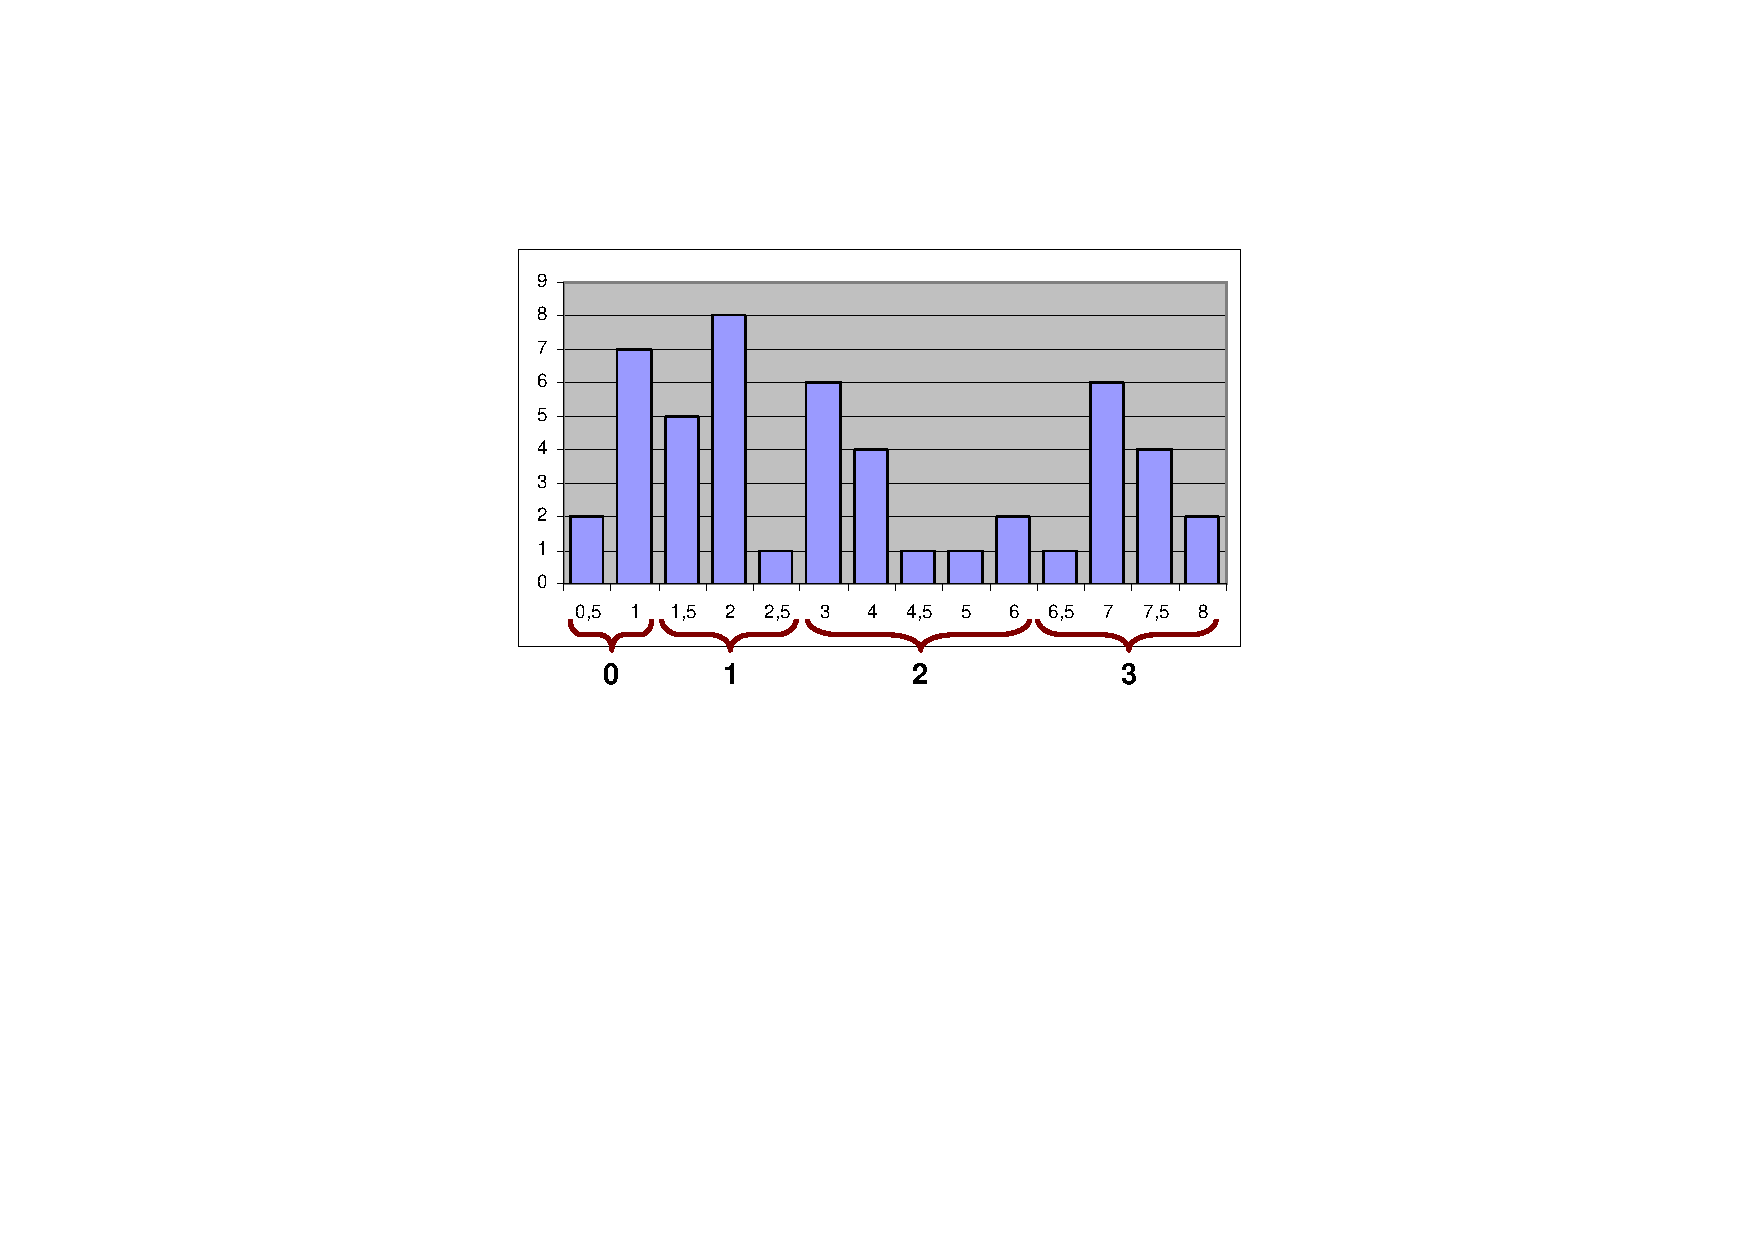
\includegraphics[angle=-90, width=0.6\hsize]{ranking_histogram}}
\caption{Frequencies of the seriousness ranking.}
\label{img:ch40_ranking_histogram}
\end{figure}

Values of the overall seriousness ranking attribute were stated from ``a general impression'' made by the texts with respect to particular attributes. %(Figure~\ref{img:attributes_description}). 
The values have evolved to 14 distinct values in the range from 0.5 to 8. 
A histogram with frequencies of all these values is in Figure~\ref{img:ch40_ranking_histogram}.
We divided the values into four approximately equipotent groups 
(see in Figure~\ref{img:ch40_ranking_histogram}) 
and these groups determine the target class attribute of the classification task. 
%and logic rules were learned for each group separately\footnote{We do not have a binary rule, which would return an exact value of the rating, but we have one ``true/false'' rule for each of the four categories.}.






\subsection{Classification Datasets from UCI ML Repository} \label{sec:ch40_uci_datasets}

UCI Machine Learning Repository\footnote{\url{http://archive.ics.uci.edu/ml/index.html}} \citep{biblio:UCI} is a large archive of machine learning datasets collected at the University of California, Irvine. Several classification datasets were selected and used in the evaluation of the Fuzzy ILP Classifier, see in Section~\ref{sec:eval_fuzzy_uci}.
The list of selected datasets can be found in Table~\ref{tab:UCI_datasets}. All the datasets are monotonizable (the target attribute can be naturally ordered), so the fuzzy classifier could take advantage of that.


\begin{table}
	\centering
	\begin{threeparttable}
		\begin{tabular}{lll}
shortcut & name & url suffix\tnote{a}\\
\hline
car    & Car Evaluation  & \href{http://archive.ics.uci.edu/ml/datasets/Car+Evaluation}{\ttfamily Car+Evaluation}\\
wine\tnote{b} & Wine Quality  & \href{http://archive.ics.uci.edu/ml/datasets/Wine+Quality}{\ttfamily Wine+Quality}\\
cmc    & Contraceptive Method Choice  & \href{http://archive.ics.uci.edu/ml/datasets/Contraceptive+Method+Choice}{\ttfamily Contraceptive+Method+Choice}\\
tae    & Teaching Assistant Evaluation  & \href{http://archive.ics.uci.edu/ml/datasets/Teaching+Assistant+Evaluation}{\ttfamily Teaching+Assistant+Evaluation}\\
pop    & Post-Operative Patient  & \href{http://archive.ics.uci.edu/ml/datasets/Post-Operative+Patient}{\ttfamily Post-Operative+Patient}\\
nurs   & Nursery  & \href{http://archive.ics.uci.edu/ml/datasets/Nursery}{\ttfamily Nursery}\\
\hline
		\end{tabular}
		\begin{tablenotes}
			\item [a] The prefix is: \url{http://archive.ics.uci.edu/ml/datasets/}
			\item [b] Only red wine part of the dataset was used.
		\end{tablenotes}
		\caption{Classification datasets selected form the UCI ML Repository.} \label{tab:UCI_datasets}
	\end{threeparttable}
	
\end{table}



